\documentclass[../main/main.tex]{subfiles}
\begin{document}
%\dominitoc
%\faketableofcontents
\setcounter{chapter}{1}
\chapter{Cosmologie avec les Supernovae de type Ia}\label{ch:snia}

\minitoc
\vspace{2cm}

Tycho Brahé, un astronome considéré comme l'un des pioniers de l'astronomie
observationnelle moderne, observe en 1572 l'apparition soudaine d'une
nouvelle étoile. Cet objet est alors nommé \textit{nova}, terme latin
signifiant \textit{nouveau}. En de rares occasions au cours des
civilisations, les astronomes ont pu être témoins de tels évènements,
parfois visibles même en plein jour.

En 1934, Walter Baade et Fritz Zwicky introduisent le terme de
\textit{supernova} pour nommer les plus brillants de ces évènements,
pouvant être plus lumineux que leur galaxie hôte.

Cet évènement transitoire pouvant durer plusieurs semaines à plusieurs
mois est la conséquence de la mort d'une étoile. Suivant le processus
d'explosion, ces supernovae (SNe) sont classées par type, discernables
par leurs propriétés spectrales.

Les supernovae de type Ia (SNeIa) sont un type particulier de ces
objets, ayant la particularité d'avoir une faible dispersion en
luminosité. Cette propriété leur vaut le titre de chandelles standard,
et sont ainsi utilisés comme indicateur de distance dans les études
cosmologiques. 

Nous introduisons dans ce chapitre les différents types de supernova et
les caractéristiques permettant de les classifier. Nous nous
concentrerons ensuite sur l'étude des SNeIa et leur utilisation dans la
cosmologie moderne.

\newpage

\section{Zoologie et classification des supernovae}

\subsection{Caractéristiques principales}

Les supernovae sont principalement classifiées suivant leurs
caractéristiques spectrales. C'est en 1941 que R. Minkowski
\citep{Minkowski1941} remarqua pour la première fois l'existance de deux
types différents de SNe. Le premier type (I) est caractérisé par
l'absence d'hydrogène, et le second type (II) en contient.
Près d'un demi siècle plus tard, \citet{Elias1985} apporte une
classification plus fine des types I, séparant les SNe possédant une importante
raie du silicium (les SNeIa) des Ib et des Ic. Les
types Ib sont caractérisés par la présence d'une raie d'hélium, et les
Ic par l'absence de silicium et une faible quantité d'hélium présente
dans leur spectre. La Figure~\ref{fig:snetypes} illustre la forme du
spectre de différents types de supernovae, indiquant les raies
d'émissions et d'absorption caractéristiques de chacun.


\subsection{Mécanismes d'explosion}
La physique des SNeIa est considérablement différentes des autres types
de SN. En effet, les types Ib/c et les types II proviennent d'un
mécanisme d'\textit{effondrement de coeur}, c'est à dire d'implosion
gravitationnelle. Le progéniteur de ces évènements (étoile qui a donné
naissance à la supernova), est une étoile massive de plus de $8$ masses solaires
\citep{Heger2003}. Après avoir consommé tous les éléments légers
composant son coeur, celui ci s'effondre sur lui même jusqu'à ce que la
force d'intéraction forte le stoppe. La pression radiative n'étant plus
à même de contrer les effets gravitationnels, les couches externes de
l'étoile tombe vers le centre et rebondissent sur le coeur alors
incomprésible. L'onde de choc provoque l'explosion de l'étoile en
supernova.
La nature du résidu de l'explosion dépend de la masse du progéniteur. Si
cette masse était de moins de $30\Msun$, le résidu sera une étoile à
neutrons, dans le cas contraire un trou noir se formera.
Pour ces supernovae, la luminosité et son évolution temporelle dépend
fortement de la composition du progéniteur et de sa masse
initiale. Ces fortes variabilités n'en font pas de bons candidats en
tant que chandelles standard pour des mesures de distance.

Les supernovae de type Ia en revanche auraient pour origine l'explosion
thermonucléaire d'une naine blanche. Cet objet se créé lorsque la masse d'une étoile n'est pas
suffisante ($<3\Msun$) pour générer la température nécéssaire à la
fusion du carbone ($\sim10^{9}K$). Après la fusion des éléments
légers du coeur, une masse inerte composée de carbone et d'oxygène va se
former. La naine blanche est le résidu d'une telle étoile suite à l'expulsion des couches externes (générant au passage une
nébuleuse planétaire).
L'intégrité de cet astre est entièrement assurée par l'équilibre entre
la gravitation et sa pression interne (pression de dégénerescence des
électrons), dont la physique impose une masse maximale de
$\sim1.44\Msun$ appelée \textit{masse de Chandrasekhar} \citep{Chandrasekhar}.
Quand cette limite est atteinte, la pression du gaz d'électrons
dégénérés n'est plus suffisante pour retenir les forces de pression
gravitationnelles. La température monte alors suffisamment pour
permettre la fusion du carbone, ce qui entraîne la combustion totale de
l'étoile: une supernova de type Ia.

La faible dispersion en luminosité
des SNeIa associée à la présence de silicium et de calcium dans leur spectre
sont des éléments favorisant ce scénario \citep{Hoyle1960}. En effet,
les fusions du carbone et de l'oxygène qui composent la naine blanche
produisent du silicium et du calcium, expliquant leur présence dans les
spectres des SNeIa. L'explosion du progéniteur se déroulant toujours
dans les mêmes conditions, la quantité et la nature des combustibles sont
similaires d'une explosion à l'autre, expliquant la faible dispersion en
luminosité. Enfin, l'absence d'hélium et d'hydrogène dans le spectre
d'une SNIa contrairement aux autres type s'explique par l'absence de ces
éléments dans une naine blanche carbone oxygène.


\begin{figure}[ht]
  \begin{minipage}[c]{0.59\textwidth}
    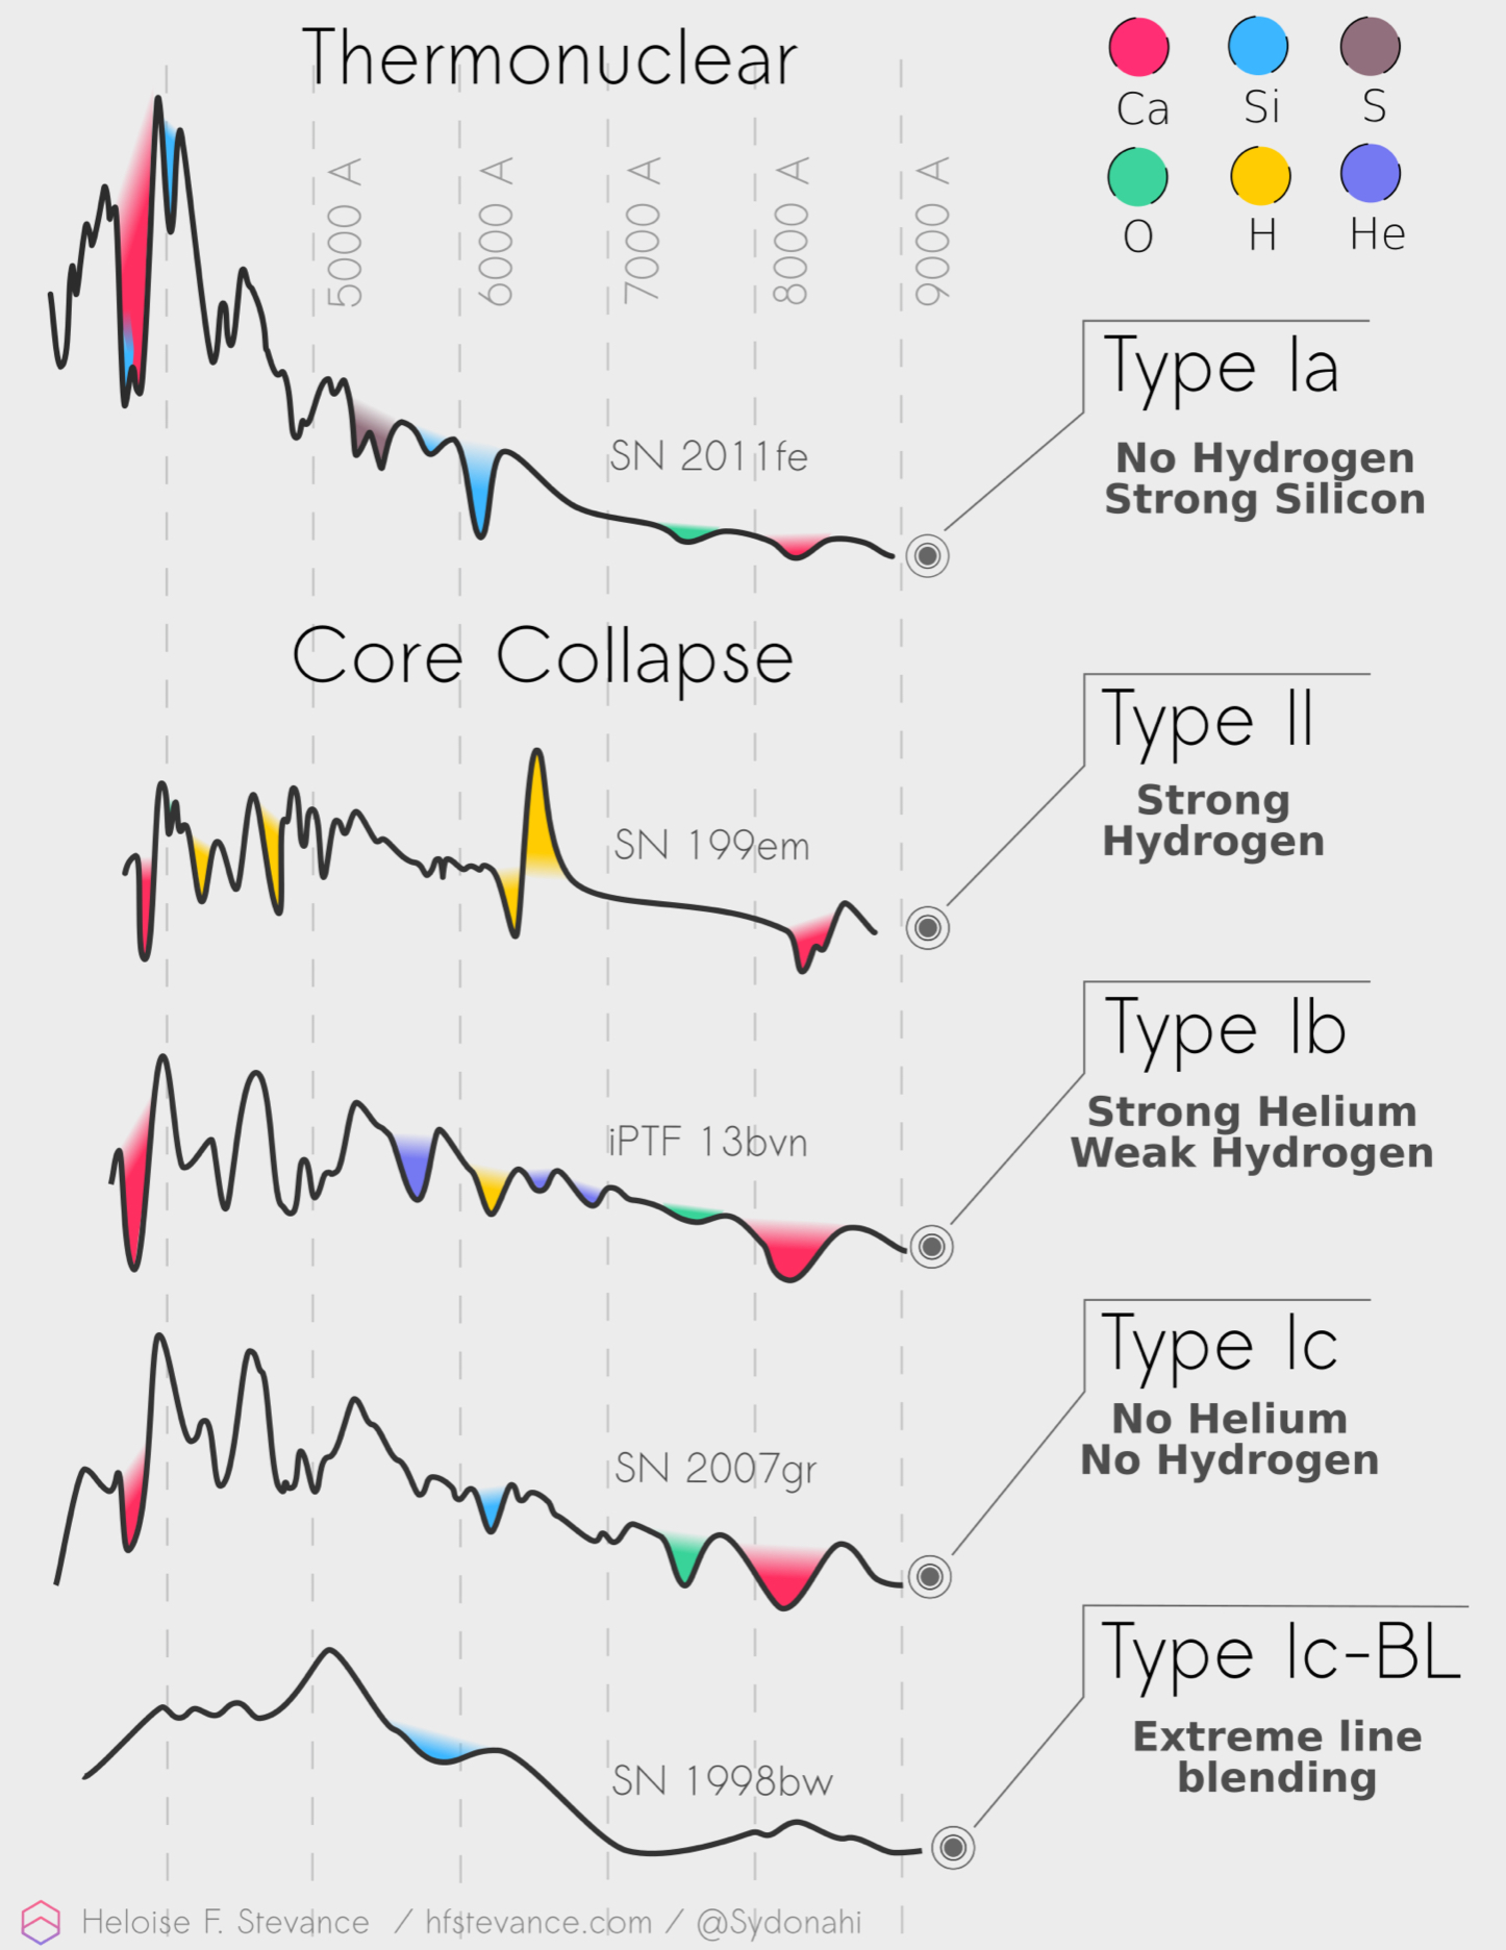
\includegraphics[width=\textwidth]{../figures/01bis_sne/snetype.pdf}
  \end{minipage}\hfill
  \begin{minipage}[c]{0.4\textwidth}
    \caption[Spectre de différents types de supernovae.]{Spectre de
      différents types de supernovae. Image de H. Stevance\footnote{\url{https://github.com/HeloiseS/Graphics}}}\label{fig:snetypes}
  \end{minipage}
\end{figure}

\section{Standardisation des SNeIa}

L'évolution temporelle de la luminosité des SNeIa, leur courbe de
lumière, montre une très forte homogénéité notamment au pic de
luminosité. Cette particularité, leur donnent des propriétés de
chandelles standard, permet d'utiliser les SNeIa comme
indicateurs de distance.

\subsection{Chandelles standardisables}
Les SNeIa n'étant pas observées dans la Voie Lactée, une calibration
de leur luminosité est au préalable effectuée à l'aide d'un autre estimateur de
distance extra-galactique.
Un de ces calibrateurs sont les céphéides, étoiles jeunes présentant des
pulsations radiales régulières. Ces pulsations entraînent une
variabilité de leur rayon et de leur température de façon périodique, et
ainsi de même sur leur luminosité. \citet{Leavitt1908, Leavitt1912} ont
ainsi montré que la magnitude absolue des céphéides était
proportionnelle à leur période de pulsation. En observant de telles
étoiles dans notre galaxie, les coefficients de proportionnalité de
cette relation ont eux même pu être calibrés par une autre méthode indépendante
de mesure de distance, la parallaxe stellaire.

En utilisant des céphéides dans des galaxies proches
($\sim30$Mpc) ayant accueilli une SNIa, il est alors possible de
calibrer leur distance et donc leur luminosité
intrinsèque. \citet{Saha1999} trouvent par exemple avec un échantillon
de $8$ SNeIa une valeur moyenne de
la magnitude absolue (au pic) dans la bande V de:
\begin{equation}
  \label{eq:51}
  \langle M_{V}\rangle=-19.48\pm0.07 
\end{equation}
et \citet{Hamuy1995}  montrent une
dispersion de luminosité de l'ordre de $\sigma_{M_{V}}\leq0.5$ mag.
Nous parlons finalement en réalité de chandelles \textit{standardisables}, avec une
certaine variabilité en luminosité qui doit être corriger. L'étude des
courbes de lumière a permis de déceler des corrélations fortes entre la
luminosité au maximum et certains paramètres des SNeIa que nous
définierons plus loin, permettant
de réduire considérablement cette dispersion. 

\subsection{Courbes de lumière et spectres de SNeIa}

La courbe de lumière d'une SNIa est obtenue en observant son évolution en magnitude au cours du temps
dans une bande photométrique donnée. De façon générale pour ce type de
supernova, nous observons après l'explosion une augmentation rapide\footnote{De
l'ordre d'une diminution de $3$ à $6$ mag suivant la bande photométrique} de
luminosité sur un quinzaine de jours jusqu'au pic de
luminosité. La phase $0$ de la courbe de lumière est définie comme le
pic de luminosité dans la bande photométrique $B$.

Après le pic de luminosité, la décroissance s'effectue en deux phase. La
première, abrupte, ne dure que quelques jours et est dominée par la
désintégration $^{56}\text{Ni}\rightarrow \, ^{56}\text{Co}$. La seconde
phase de décroissance de luminosité est plus douce et s'étale sur
plusieurs dizaines de jours, et est dominée par la désintégration
$^{56}\text{Co}\rightarrow \, ^{56}\text{Fe}$.

La Figure~\ref{fig:specevolsnia} \citep[extraite de][]{Pereira2013}, expose un exemple d'évolution temporelle du spectre
d'une SNIa \citep[SN2011fe, découverte par][]{Nugent2011} où nous
apercevons clairement la variabilité chimique de la supernova. Entre les
phases ($-15$,$+15$) jours, la
raie d'absorption du silicium est la caractéristique principale du
spectre. Elle s'aténue progressivement dans les mois qui suivent
l'explosion, et les raies d'émission du fer deviennent à leur tour la caractéristique
principale du spectre. Cette
SNIa a été observée par le télescope de l'Université de Hawaï avec le
spectrographe à champs intégral SNIFS \citep[SuperNova Integrated Field
Spectrograph][]{SNIFS2004} de la collaboration \textit{Nearby Supernova
  Factory} \citep{Aldering2002}.
On remarque le maximum de luminosité autour de $4000$\AA, et le
fait que la majorité de l'énergie de la SNIa est émise dans le proche
infrarouge, le visible et le proche ultraviolet. 

Pour cette même supernova, nous montrons les courbes de lumière
reconstruites dans les bandes $U$, $B$, $V$, $R$, et $I$. Nous pouvons
clairement apercevoir la montée rapide du flux jusqu'au maximum de
luminosité (pouvant survenir à une date différente suivant la bande
considérée), suivi de la décroissance du flux. Nous pouvons également
relever la présence d'un second maximum environ un mois après le premier
dans les bandes infrarouges.

\begin{figure}[ht]
  \centering
  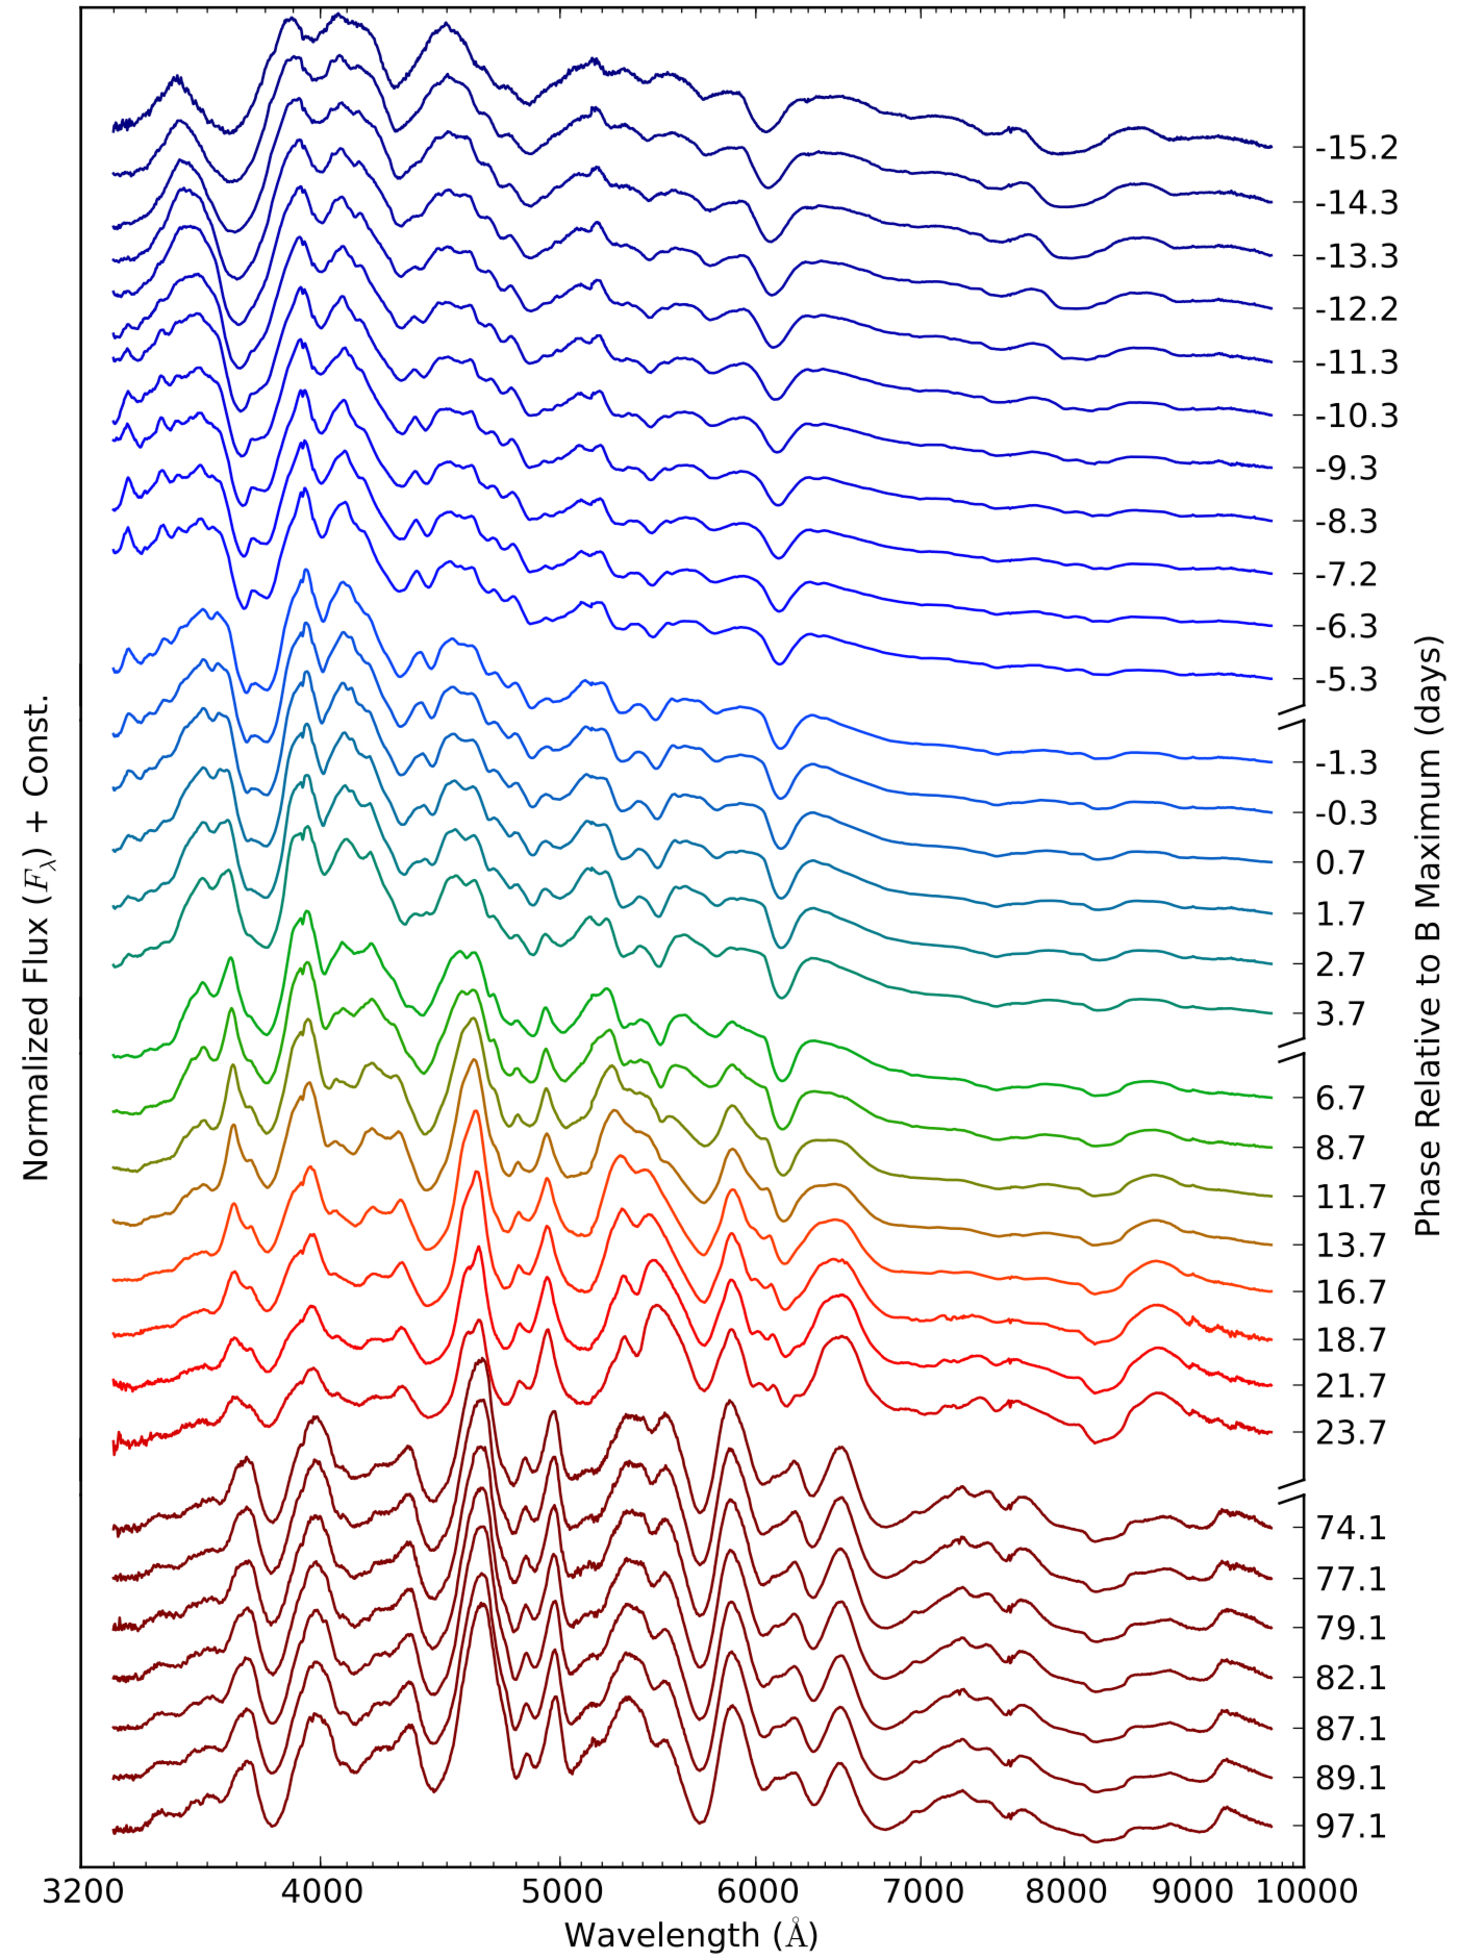
\includegraphics[width=0.77\textwidth]{../figures/01bis_sne/sniaspecevol.pdf}
  \caption[\'Evolution temporelle du spectre de la SNIa
  SN2011fe.]{\'Evolution temporelle du spectre de la SNIa SN2011fe entre
  $-15$ et $+100$ jours relativement à la phase $0$ (pic de luminosité
  dans la bande $B$). Figure de \citet{Pereira2013}, réalisée par la
  collaboration SNFactory.}
  \label{fig:specevolsnia}
\end{figure}

\begin{figure}[ht]
  \centering
  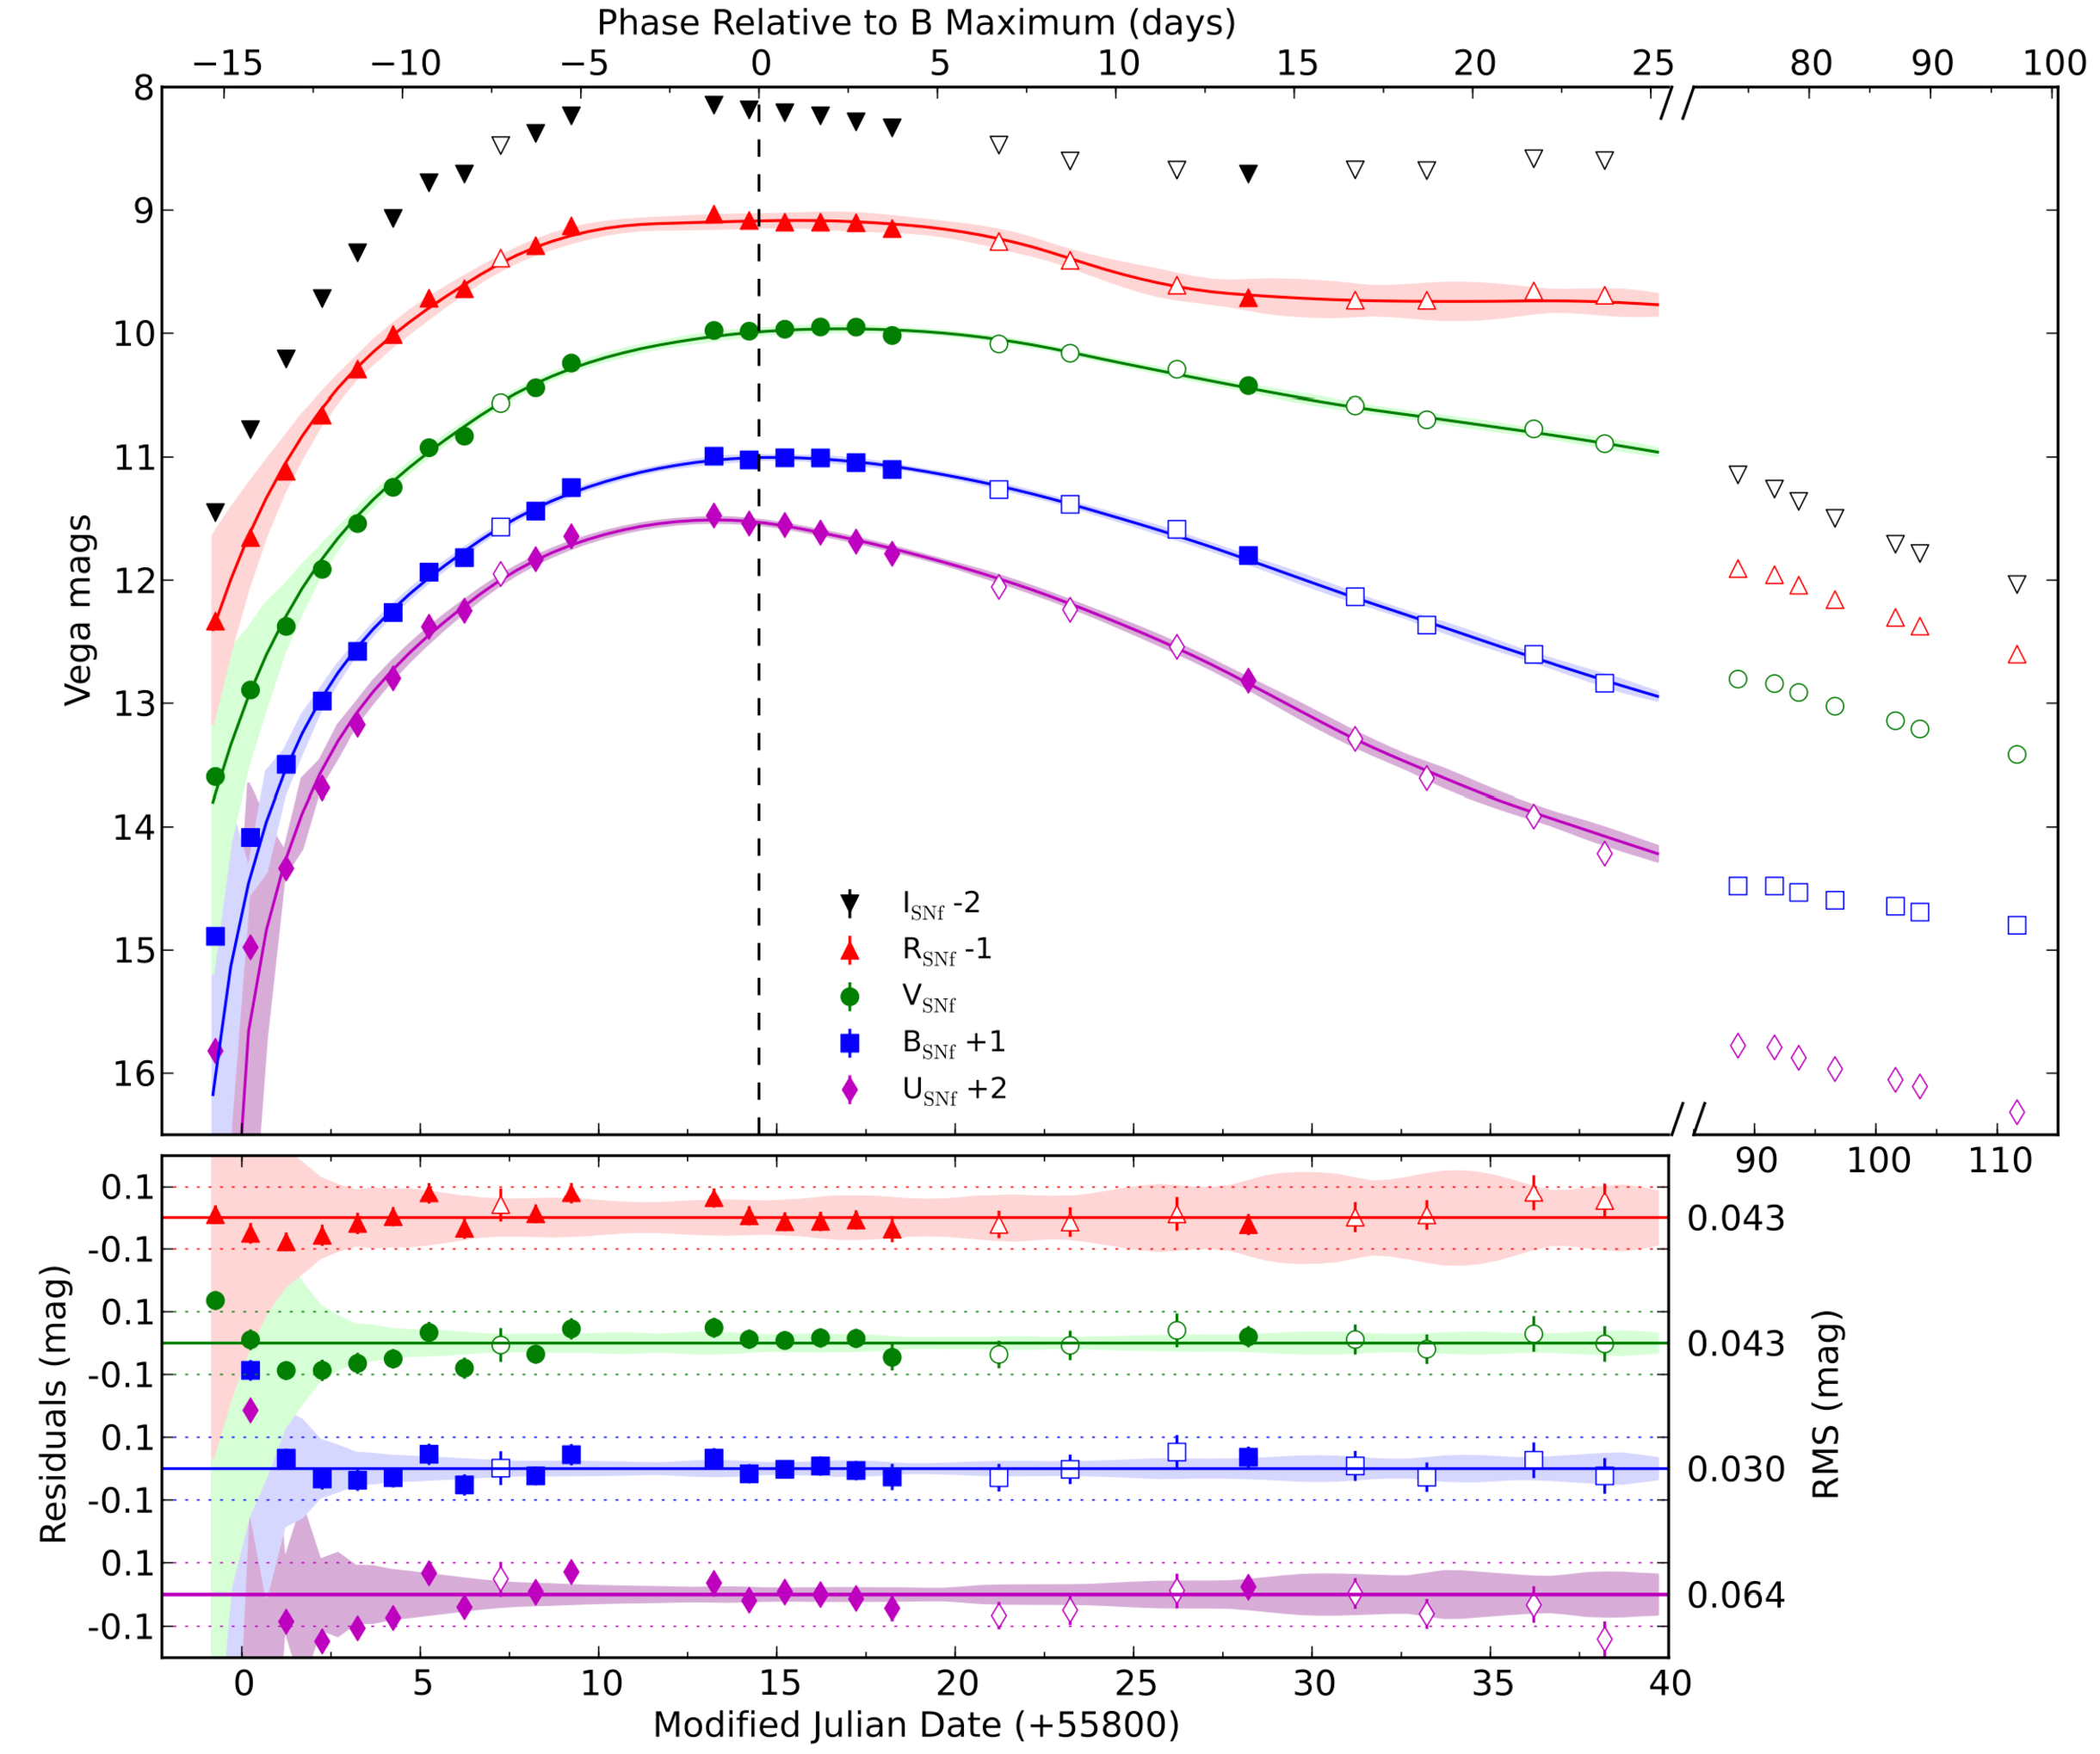
\includegraphics[width=0.9\textwidth]{../figures/01bis_sne/lightcurvesnpereira.pdf}
  \caption[Courbe de lumière de la SNIa
  SN2011fe.]{Courbe de lumière de la SNIa SN2011fe entre
  $-15$ et $+100$ jours relativement à la phase $0$ (pic de luminosité
  dans la bande $B$) et dans les bandes $UBVRI$. Les courbes indiquent
  l'ajustement effectué avec le modèle SALT2 (Sec~\ref{ssec:salt2}). Le
  graphique du bas montre les résidus entres les mesures photométriques
  et le modèle ajusté. Les bandes de couleurs indiquent les incertitudes
  du modèle. Figure de \citet{Pereira2013}, réalisée par la
  collaboration SNFactory.}
  \label{fig:lightcurvesnpereira}
\end{figure}

\clearpage
\subsection{Propriétés des courbes de lumière}


\subsubsection*{La couleur}

La pente générale du spectre d'un objet astrophysique est caractérisée
par sa couleur. Ce paramètre peut être obtenu en regardant la différence
de magnitude entre deux bandes photométriques. Pour une SNIa par
exemple, nous pouvons évaluer la quantité ($B$-$V$)$_{0}$, correspond à
la différence de magnitude dans les bandes $B$ et $V$ de son référentiel
et à la phase $0$ (maximum de luminosité).

Cette prorpiété peut varier d'un SNIa à une autre. Cette fluctuations
peut-être de nature extrinsèque, causée par l'extinction due à la
poussière présente dans la galaxie hôte de la SN et le long de la ligne
de visée, ou encore de nature intrinsèque comme une possible variabilité
du progéniteur.
Pour une SNIa $i$, on définit l'excès de couleur $c$ comme la différence
entre sa couleur et celle moyenne de l'échantillon:
\begin{equation}
  \label{eq:color}
  c=(B-V)^{i}_{0}-\langle(B-V)_{0}\rangle
\end{equation}

Par défnition, les SNeIa ayant un excès de couleur négatif seront plus
bleues que la moyenne, et celles ayant un excès de couleur positif plus
rouges.

\subsubsection*{L'étirement temporelle}

Bien que la forme générale de la courbe de lumière des SNeIa soit très
homogène, on peut observer (après correction de la dilatation temporelle
causée par le redshift) des variations sur le temps de montée
jusqu'au maximum de luminosité ainsi que sur la phase décroissante.

La première description quantitative de cette dilatation résiduelle a
été apportée par \citet{Phillips1993},
introduisant la quantité $\Delta m_{15}(B)$ définit comme la différence de
magnitude apparente dans la bande $B$ entre le maximum de luminosité
(phase $0$) et la phase $+15$ jours.

L'étirement temporelle telle qu'utilisée aujourd'hui est introduit
quelques années plus tard par \citet{Perlmutter1997}. Ce nouveau
paramètre $s$, appelé \textit{stretch}, correspond à un facteur
correctif par lequel il faut dilater l'axe temporel de la courbe de
lumière d'une SNIa pour qu'elle se superpose à la courbe de lumière
moyenne d'un échantillon.
\subsubsection*{Maximum de luminosité}

Enfin la luminosité au maximum est la principale prorpiété des SNeIa, car
c'est à partir de cette mesure que la distance est extraite. 
Cette luminosité, exprimée par convention dans la bande $B$, présente cependant une dispersion intrinsèque de
l'ordre de $\sim40\%$ \citep{Hamuy1996}. Nous allons voir comment il est
possible de réduire cette dispersion, de par l'existence de corrélation
entre ce maximum de luminosité, et la couleur et le stretch. 
\clearpage
\subsection{Modèle \textit{Spectral Adaptive Light-curve Template 2} (SALT2)}\label{ssec:salt2}

\subsubsection{Corrélations}

Nous montrons dans la Figure~\ref{fig:lc_jla} les courbes de lumière
dans la bande $B$ de SNeIa à bas redshift ($z<0.08$). Ces données
photométriques ont été acquises au \textit{Whipple Observatory of the
  Harvard- Smithsonian Center for Astrophysics}
\citep[CfA3,][]{Hicken2009} et utilisées pour l'analyse \textit{Joint Light-curve Analysis}
\citep[JLA,][]{Betoule2014}.  On notera la dispersion en luminosité absolue de
l'ordre de $\sim40\%$, mais surtout l'évidence de la corrélation entre
la forme des courbes de lumière, le stretch et la couleur. 

\begin{figure}[ht]
  \centering
  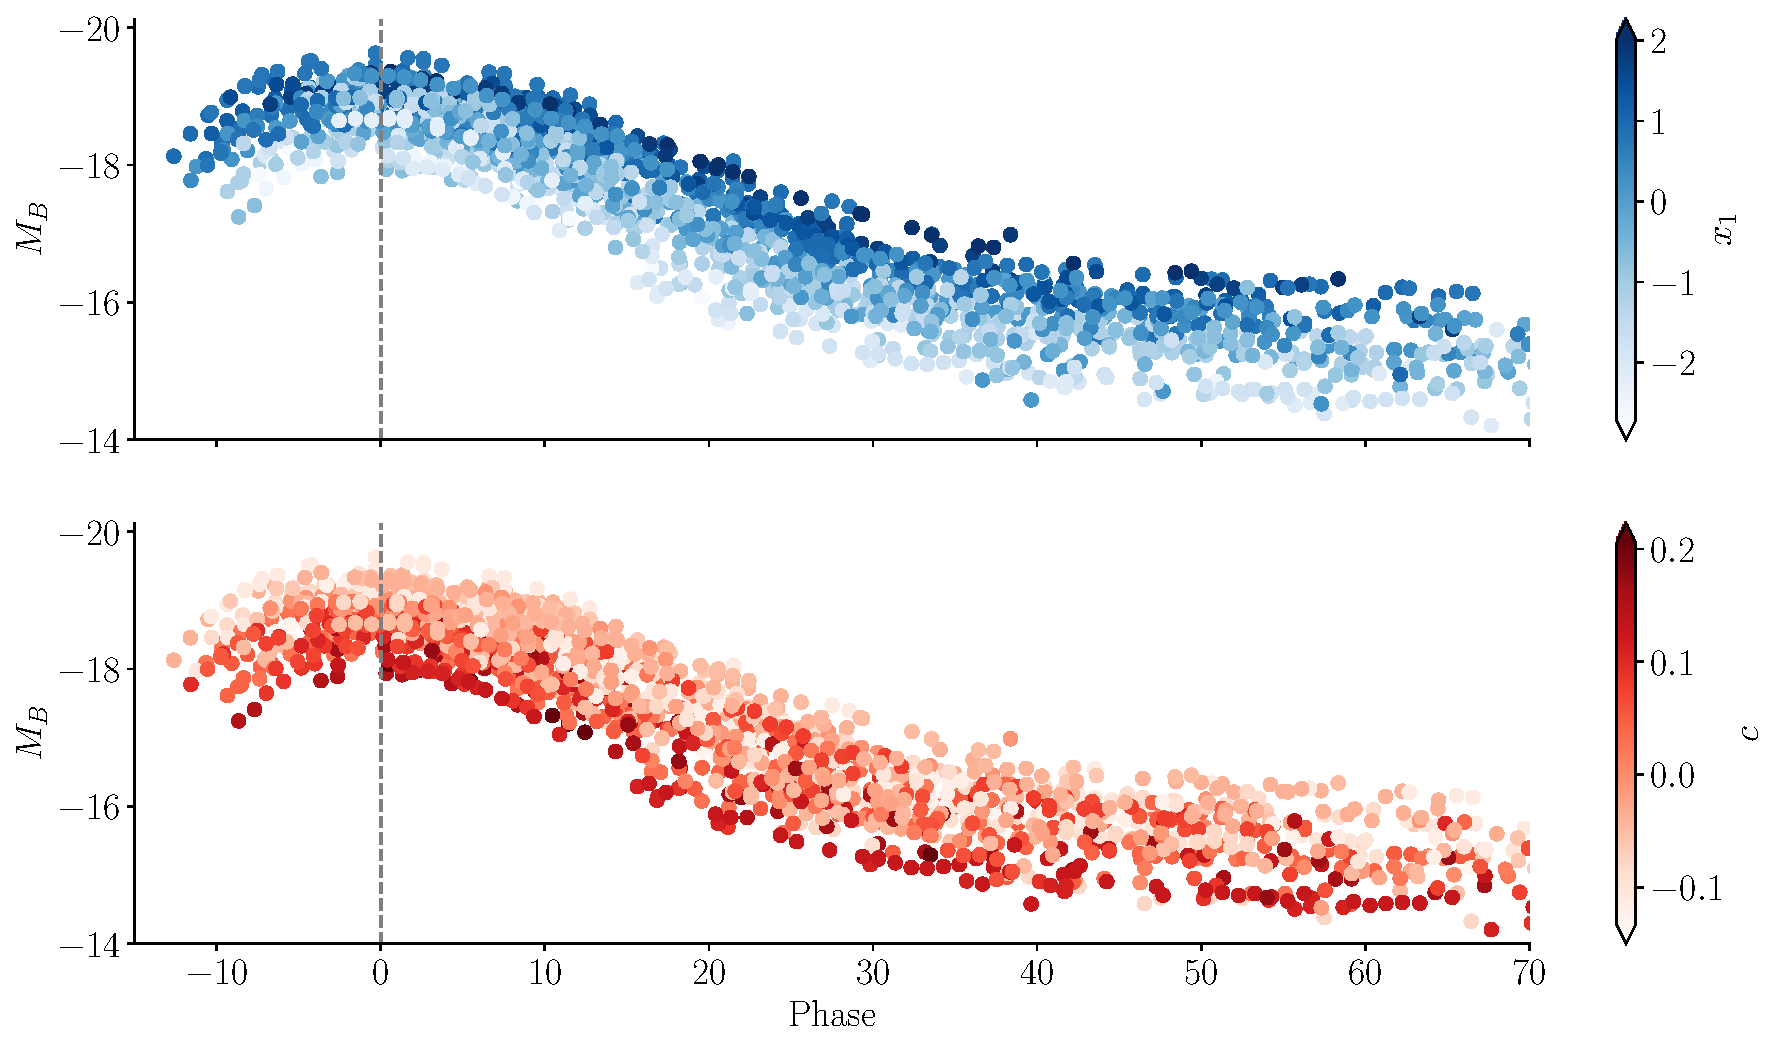
\includegraphics[width=0.99\textwidth]{../figures/01bis_sne/lc_JLA.pdf}
  \caption[Courbes de lumière de SNeIa à bas redshift de JLA.]{Courbes
    de luminosité absolue de SNeIa à bas redshift de JLA dans la bande $B$ .La ligne verticale correspond à la
    phase $0$, exprimée en jours sur l'axe des abscisses. L'axe des
    ordonnées est inversée pour que les fortes luminosité soient vers le
    haut. \emph{En haut} le code
    couleur indique la valeur de l'étirement temporel $x_{1}$. \emph{En
      bas} nous montrons les mêmes courbes de lumière mais avec
    l'information de la couleur $c$. Nous notons la dispersion en
    luminosité de l'odre de $0.5$ mag, et surtout la variabilité avec le
  stretch et la couleur.}
  \label{fig:lc_jla}
\end{figure}

La variabilité des courbes de lumière avec la couleur $c$ des SNeIa fut
initialement mis en évidence par \citet{Hamuy1996} puis par \citet{Tripp1999} sur l'échantillon de
SNeIa du Calan-Tololo. Les SNeIa les plus bleues s'avère être plus
lumineuses, effet appelé \textit{bluer-brighter}. Avec la définition de
l'excès de couleur, cela correspond donc à un paramètre $c<0$.

L'autre corrélation clairement visible dans la
Figure~\ref{fig:specevolsnia} est celle du
stretch $x_{1}$, introduite par \citet{Phillips1993} avec la quantité
$\Delta m_{15}$ puis en temps que facteur correctif de l'étirement
temporelle par \citet{Perlmutter1997}. Cette corrélation montre que les
SNeIa dont la courbe de lumière évolue lentement ($x_{1}>0$) sont plus
lumineuses (\textit{slower-brighter}).

Nous montrons dans la Figure~\ref{fig:colorstretch_corr_JLA} l'évolution
du maximum de luminosité dans la bande $B$ avec la couleur et le stretch
pour les mêmes SNeIa que dans la Figure~\ref{fig:specevolsnia}. Ces deux
corrélations, intuitives en visualisant les courbes de lumière, sont ici
clairement explicitées. 

\begin{figure}[ht]
  \centering
  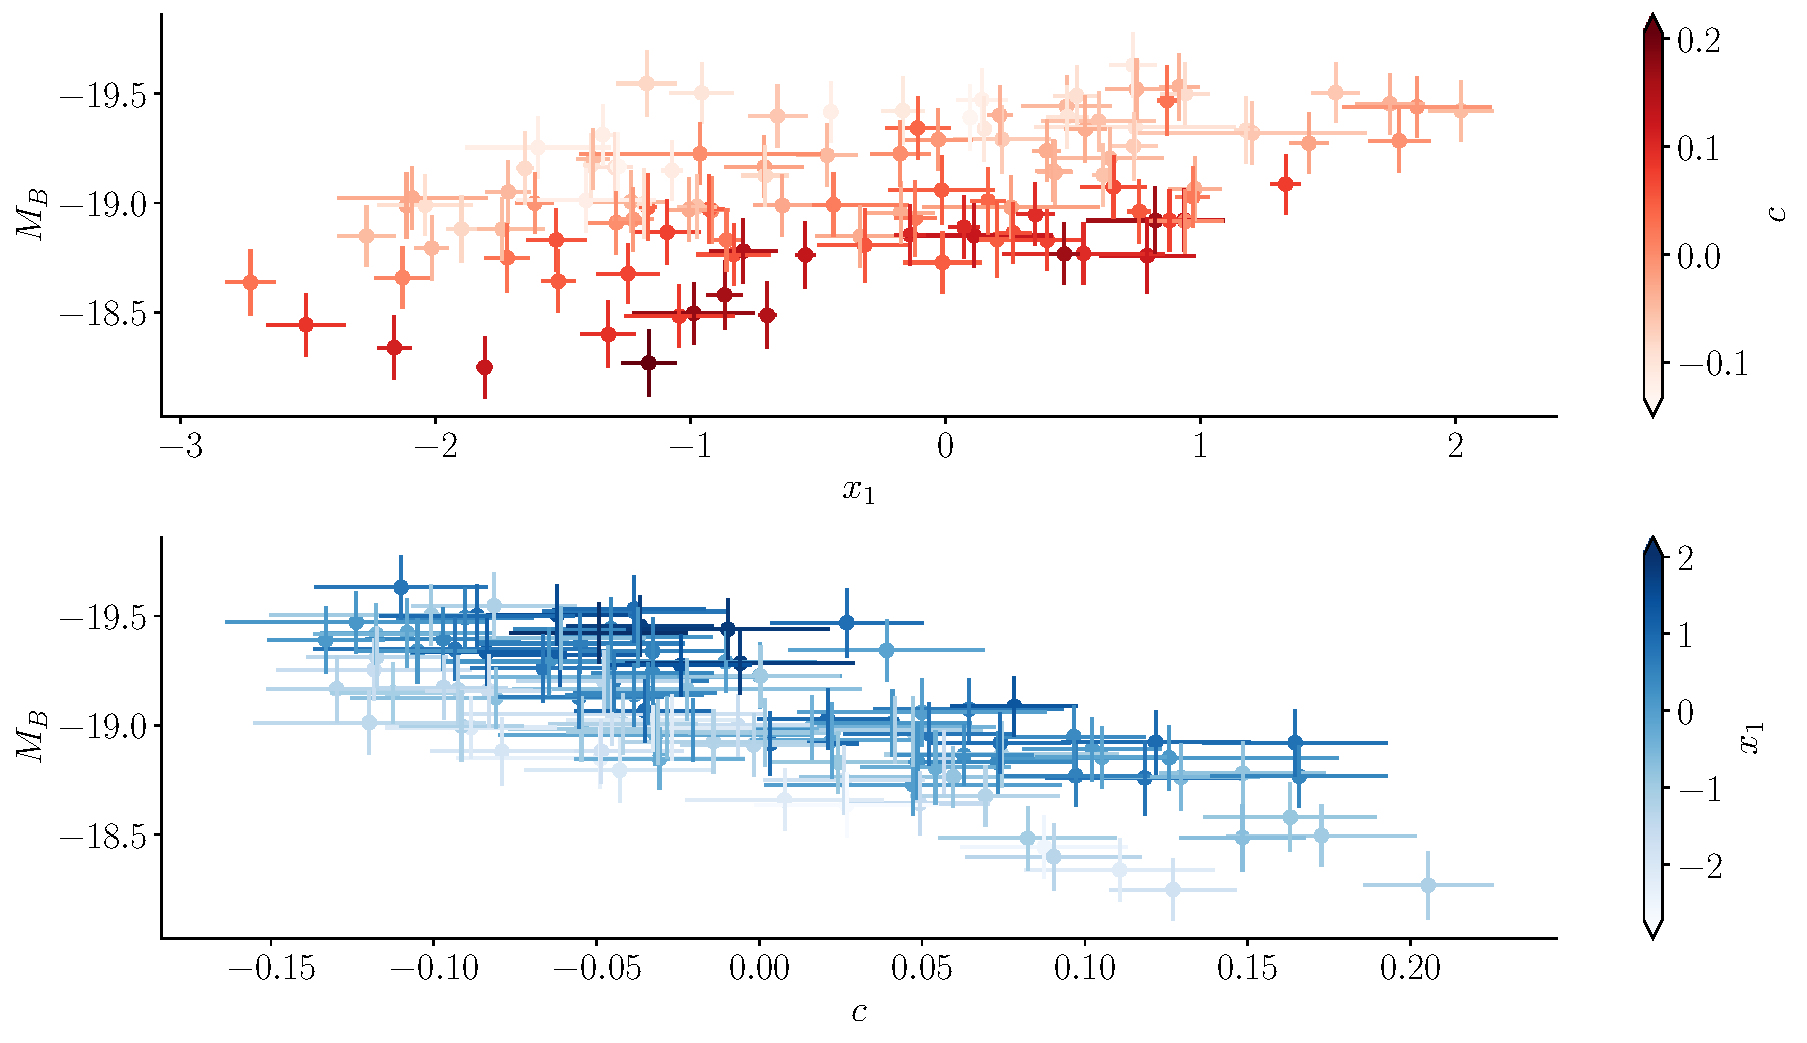
\includegraphics[width=0.99\textwidth]{../figures/01bis_sne/colorstretch_corr_JLA.pdf}
  \caption[\'Evolution du maximum de luminosité avec le stretch et la
  couleur pour les SNeIa à bas redshift de JLA.]{\'Evolution du maximum de luminosité avec le stretch et la
  couleur pour les SNeIa à bas redshift de JLA dans la bande
  $B$. Le graphe \emph{en haut} montre l'évolution du pic de magnitude
  avec le stretch. L'échelle de
    couleur en rouge indique la couleur $c$ associée à chaque SNIa. De
    même, nous montrons \emph{en
      bas} les corrélations avec la couleur $c$, où le stretch est
    indiqué avec l'échelle de couleur bleue.}
  \label{fig:colorstretch_corr_JLA}
\end{figure}


\subsubsection{Standardisation et SALT2}

La standardisation des SNeIa se fait donc en déterminant au préalable
les paramètres de stretch et de couleur. Une des méthodes existantes est
la modélisation des courbes de lumière avec le modèle \textit{Spectral
  Adaptive Light-curve Template 2}
\citep[SALT2][]{Guysalt2005,Guysalt22007}, et notamment la dernière
version (\pkg{v2.4}) développée par \citet{Betoule2014}. 
Cette méthode utilise un modèle empirique de densité spectrale en
énergie (SED) au premier ordre des SNeIa au cours du temps et entraîné avec des données spectrophotométriques provenant de
SNLS et SDSS \citep{Betoule2014}. En considérant une phase $p$ et une longueur d'onde
$\lambda$, le flux observé d'une SNIa est exprimée par:
\begin{equation}
  \label{eq:saltflux}
  f(p,\lambda)=x_{0}\left[M_{0}(p,\lambda)+x_{1}M_{1}(p,\lambda)\right]\times\exp\left(c\times
    C_{L}(\lambda)\right)
\end{equation}
avec $x_{0}$ un facteur de normalisation, $M_{0}(p,\lambda)$ le SED
moyenne, $M_{1}(p,\lambda)$ la variabilité au premier ordre autour de la
séquence moyenne et $C_{L}(\lambda)$ une loi de couleur
entraînée. $x_{1}$ et $c$ sont les paramètres de stretch et de couleur.
Les paramètres \{$M_{0}$, $M_{1}$, $C_{L}$\} sont des propriétés
globales du modèle, et les paramètres \{$x_{0}$, $x_{1}$, $c$\} sont
ajustés simultanément sur les courbes de lumière dans toutes les bandes
disponibles pour une SNIa donnée. La magnitude apparente dans la bande
$B$ $m_{B}$ est ensuite déterminée par intégration de la SED du modèle
dans la bande correspondante.


La standardisation des SNeIa se fait finalement par la relation de \citet{Tripp1998}:
\begin{equation}
  \label{eq:mustandard}
  \mu  = m_{B}- M_{B}+\alpha x_{1}-\beta c
\end{equation}
avec $\mu$ le module de distance, $m_{B}$ la magnitude apparente dans la
bande $B$, $M_{B}$ la magnitude absolue standardisée au maximum,$x_{1}$
le stretch et $c$ la couleur. La magnitude absolue $M_{B}$ ainsi que les coefficients $\alpha$ et $\beta$ sont
contraints simultanément aux paramètres cosmologiques.

Ce processus permet de réduire la dispersion de la luminosité au maximum
dans la bande $B$ à seulement $15\%$ $(\sigma_{M_{B}}\approx0.15$ mag).
\section{SNeIa et cosmologie}

\subsection{Construction d'un diagramme de Hubble}

La standardisation des SNeIa permet de reconstruire ce qu'on appelle un
diagramme de Hubble, qui représente la distance luminosité en fonction
du redshift. Nous avons présenté au premier chapitre
(Figure~\ref{fig:hubble}) le tout premier diagramme de ce genre, réalisé
avec des Céphéides par Edwin Hubble, et mettant en évidence l'expansion
de l'Univers.

La construction de ces diagrammes est toujours utilisé aujourd'hui,
d'une part pour
mesurer la constante de Hubble $H_{0}$ nécessitant une calibration absolue des
SNeIa à partir d'observations conjointes avec des céphéides \citep{Riess2016}, d'autre
part pour mesurer l'accélération de l'expansion de l'Univers avec une
calibration relative des SNeIa \citep{Riess1998, Perlmutter1999,
  Betoule2014}.

On utilise pour cela la relation de \citet{Tripp1998} du module de
distance introduit plus tôt (eq~\ref{eq:mustandard}), avec la méthode de
standardisation des SNeIa. 

On rappelle que le module de distance est défini comme
$\mu=5\log_{10}(d_{L})-5$ (eq~\ref{eq:distmodulemu}), et dépend donc des paramètres cosmologiques.
On défini le module de distance théorique pour une SNIa $i$ par:
\begin{equation}
  \label{eq:mutheo}
  \mu_{th,i} = \mu_{th,i}\left(z_{i}, \Omega_{M}, w_{0}, w_{a}\right)
\end{equation}
dans le cadre d'un modèle cosmologique préalablement choisi, par exemple
ici $w_{z}$-\lcdm, Univers plat laissant libre l'équation d'état de
l'énergie sombre. 

Les paramètres du module de distance
observé (eq~\ref{eq:mustandard}) $M_{B}$, $\alpha$ et
$\beta$ sont simultanément contraints avec les paramètres cosmologiques.

On notera que dans le cadre d'un Univers supposé \textit{a priori} plat,
alors $\Omega_{M}$ et $\Omega_{DE}$ sont reliés par la relation de
fermeture ($\Omega_{M}+\Omega_{DE}=1$). Donc pour un modèle \lcdm\
($w_{0}=-1$ et $w_{a}=0$) $\Omega_{M}$ est le seule paramètre cosmologique libre.

En général la constante de Hubble $H_{0}$ est fixé. On peut en effet
facilement montrer qu'il est impossible de contraindre simultanément
$M_{B}$ et $H_{0}$. Il suffit pour cela de développer le résidu de
Hubble, c'est à dire la différence entre le module de distance observé et le
module de distance théorique pour une SNIa donnée:
\begin{align}
  \mu - \mu_{th}&= m_{B}+\alpha x_{1}-\beta c -M_{B}
  -5\log_{10}(d_{L})+5\\
  &=m_{B}+\alpha x_{1}-\beta c - M_{B} -
    5\log_{10}\left(\frac{c(1+z)}{H_{0}}\int_{z=0}^{z=z_{e}}\frac{\d z'}{E(z')}\right) +5 \\
  &= m_{B}+\alpha x_{1}-\beta c - M_{B} -
    5\log_{10}\left(f(z,\Omega_{M},w_{0},w_{a})\right) -
    5\log_{10}\left(\frac{c}{H_{0}}\right) +5\\
  &= m_{B}+\alpha x_{1}-\beta c -
    5\log_{10}\left(f(z,\Omega_{M},w_{0},w_{a})\right)
    +2.5\log_{10}(LH_{0}^{2}) + cste
\end{align}
où nous avons supposé un modèle $w_{z}$-\lcdm\ et $E(z)$ ne dépend que des
paramètres cosmologiques et du redshift (eq~\ref{eq:Ez}). La luminosité
$L$ et la constante de Hubble $H_{0}$ sont des paramètres dégénérés ne
pouvant être contraint simultanément.

Dans le cas d'une calibration absolue des Supernovae avec un autre
indicateur de distance à bas redshift comme les céphéides, il est possible de fixer
$M_{B}$ pour contraindre $H_0$ comme effectué par \citet{Riess2016}. Dans le cas où $M_{B}$ est laissé libre, et où on
s'intéresse donc aux distances relatives, alors $H_{0}$ est fixé et seuls les paramètres
cosmologiques ($\Omega_i$) sont ajustés.

L'ajustement se fait habituellement par la méthode de moindre carrés
avec la minimisation d'un $\chi^{2}$, en utilisant une matrice de
covariance comprenant les erreurs statistiques et systématiques que nous
ne détaillerons pas ici \citep[voir][]{Betoule2014}.

\subsection{Sonder l'équation d'état de l'énergie sombre avec les SNeIa}

Les SNeIa sont d'excellentes sondes cosmiques pour dériver les
paramètres cosmologiques, et plus particulièrement lorsqu'il s'agit de
sonder l'énergie sombre. Pour contraindre l'équation d'état de cette
composante, il est nécessaire d'avoir des mesures de variations
relatives de distance de luminosité en fonction du redshift.

Les supernovae sont des évènements tellement brillants (parfois plus que
leur galaxie hôte) qu'elles peuvent être détectés jusqu'à des redshift
dépassant $z=1.7$ \citep{Rubin2013, Jones2013}. L'accélération de
l'expansion de l'Univers étant un phénomène cosmologiquement récent
($z<0.5$), les mesures simultanées de distancs à bas redshift ($z\sim0.05$) et à
haut redshift ($z\sim0.8-1$) permettent de considérablement contraindre
les paramètres d'énergie sombre.

Nous illustrons cela dans la Figure~\ref{fig:evolv_DEstate}, où nous
comparons différents modèles d'équation d'état de l'énergie sombre, avec
ou sans variation temporelle, par rapport au modèle standard \lcdm\ et
mis à l'échelle de l'époque du CMB ($z\sim1000$). Les plus grandes
variations de module de distance ($\lvert\Delta\mu\rvert\sim20$mmag) se situent à bas
redshift $z<0.03$ et à $z\sim1.5$. Les précisions actuelles sur $w$ sont
de l'ordre de $5\%$, et une déviation de $2\%$ par rapport à \lcdm\ ne
représentent qu'une variation en module de distance de
$3$\textperthousand. Cet objectif est celui du \textit{Large Synoptic
  Survey Telescope} \citep[LSST;][]{LSSTbook2}, relevé
astronomique grand champ qui sera lancé en 2023 et qui permettra de
sonder les SNeIa autour de $0.2<z<1$. Une ancre à bas redshift est donc
nécessaire, et ce rôle sera probablement rempli par le relevé Zwicky
Transient Facility \citep[ZTF;][]{GrahamZTF2019,BellmZTF2019} pour
lequel nous dédions le chapitre suivant.

\begin{figure}[ht]
  \centering
  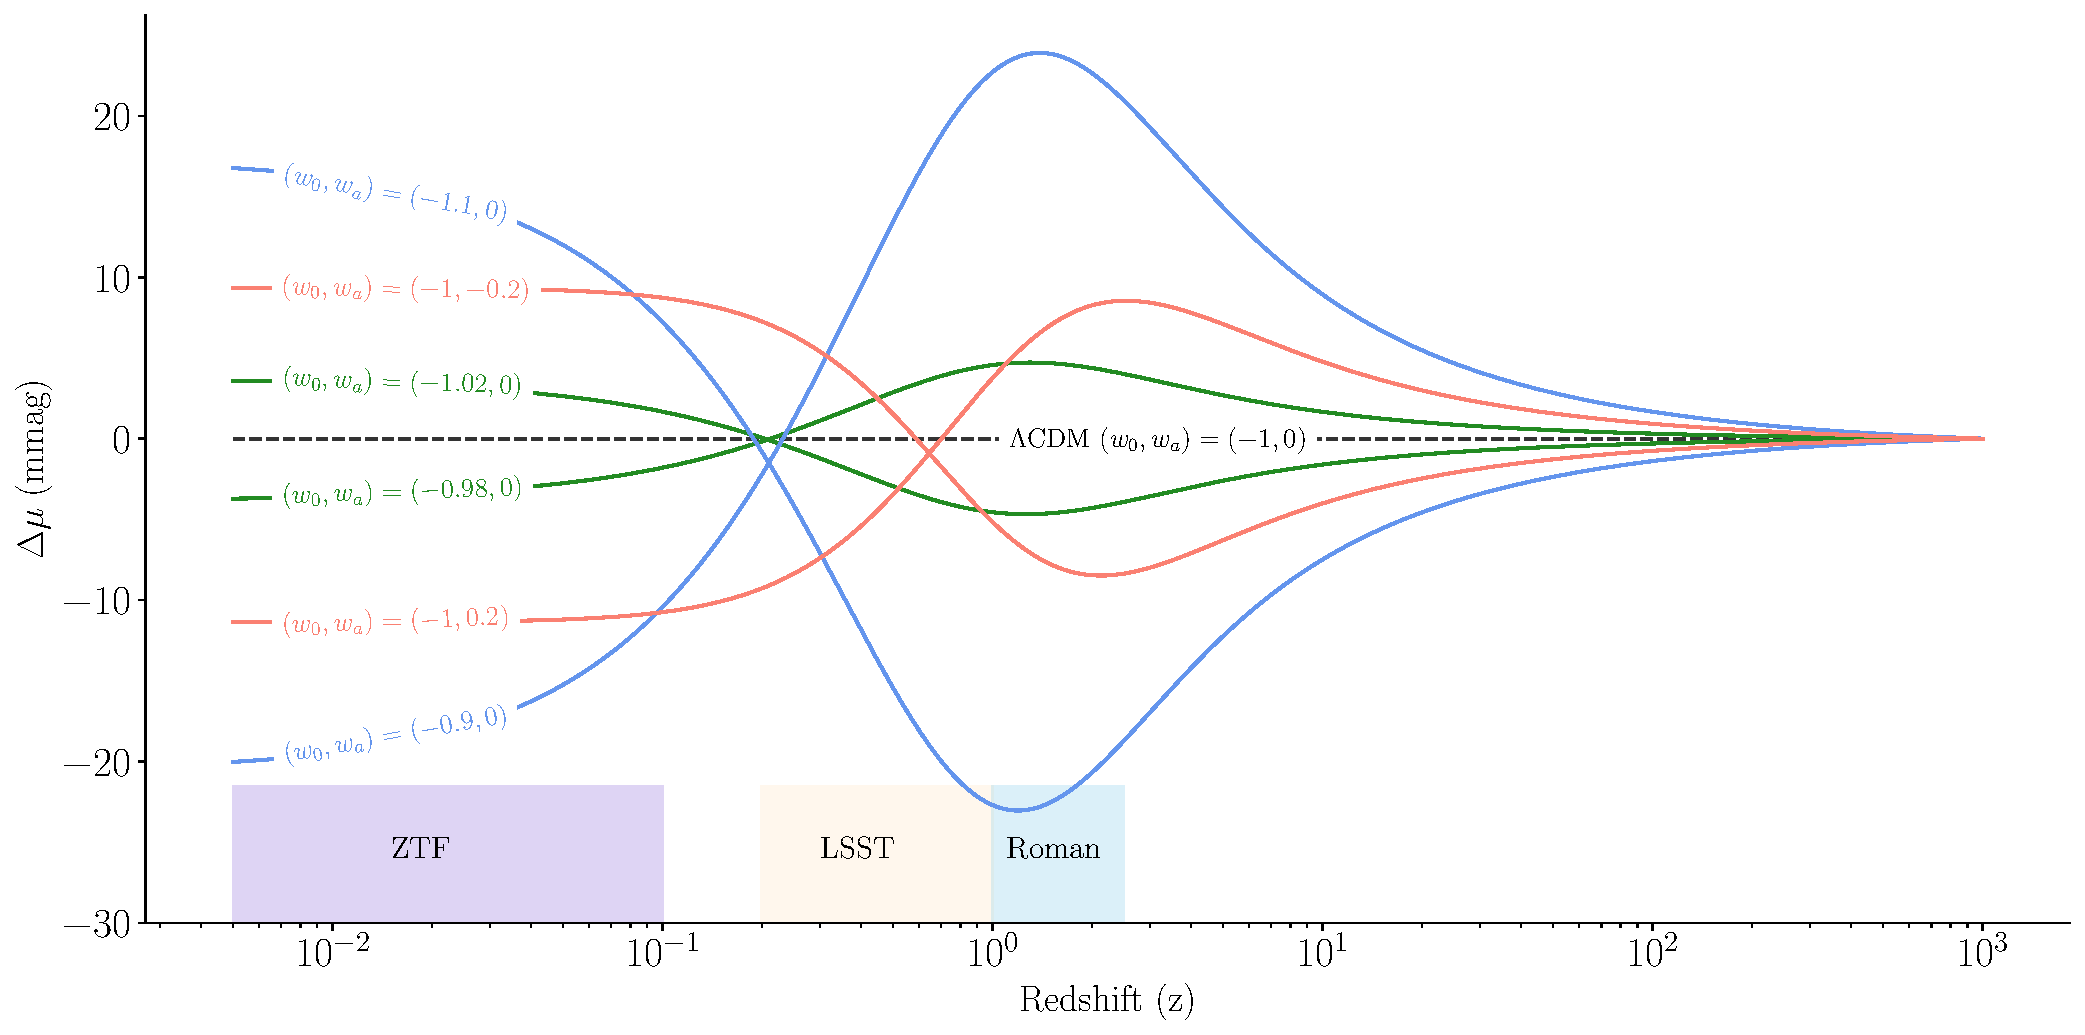
\includegraphics[width=0.99\textwidth]{../figures/01_cosmology/darkenergy_variation.pdf}
  \caption[Différence de module de distance en fonction du redshift pour
  différentes équation d'état de l'énergie sombre.]{Différence de module de distance en fonction du redshift pour
  différentes équation d'état de l'énergie sombre par rapport à \lcdm\
  ($w=0$). Les modèles sont configurés pour se rejoindre à l'époque du
  CMB. Nous illustrons ici l'importance des échantillons à bas redshitf,
et la précision nécessaire sur le module de distance pour détecter une
variation de quelques poucents de $w$. Les bandes de couleurs sur l'axe
des abscisses indiquent la profondeur en redshift des différents
relevés. ZTF est en opération depuis 2018, LSST le sera en 2023 et tout
deux sont des relevés depuis le sol. Nancy Grace Roman Telescope, spatial, sera
lancé dans le meilleur des cas en 2027, et sondera le ciel profond
jusqu'à des redshift de l'ordre de $z\sim2.5$.} 
  \label{fig:evolv_DEstate}
\end{figure}

%\bibliographystyle{../main/aa_url2}
%\bibliography{99_references}
\end{document}

%%% Local Variables:
%%% mode: latex
%%% TeX-master: t
%%% TeX-master: t
%%% End:
